\documentclass[a4paper,10pt]{article}

%%%%%%%%%%%%%%%%%%%%%%%%%%%%%%%%%%%%%%%%%%%%%%%%%%
% Los paquetes permiten ampliar las capacidades de LaTeX.                     %
%%%%%%%%%%%%%%%%%%%%%%%%%%%%%%%%%%%%%%%%%%%%%%%%%%
% Paquete para inclusión de gráficos.
\usepackage{graphicx}

% Paquete para definir la codificación del conjunto de caracteres usado
\usepackage[utf8x]{inputenc}

% Paquete para definir el idioma usado.
\usepackage[spanish]{babel}

% Paquete para introducir codigo de programacion
\usepackage{listings}

 % Para poder introducir otrod PDFs
\usepackage{pdfpages}

% Para inseratar imagenes
\usepackage{graphicx}
\usepackage{subfigure}

% Título principal del documento.
\title{\textbf{Trabajo Practico 0: Infraestructura Basica}}


% Información sobre los autores.
\author{Augusto Arturi (\#97498)\\
\texttt{turitoh@gmail.com}\\
\\
Matias Rozanec (\#97404)\\            \texttt{rozanecm@gmail.com}\\
\\
Agustin Miguel Payaslian (\#96885)\\            \texttt{payas17@hotmail.com}\\
\\
\normalsize{Grupo Nro. \# - 2do. Cuatrimestre de 2017}\\
\\
\\
\normalsize{66.20 Organización de Computadoras}\\
\normalsize{Facultad de Ingeniería, Universidad de Buenos Aires}\\
}
\date{7/09/2017}


\begin{document}

% Inserta el título.
\maketitle
% Quita el número en la primer página.
\thispagestyle{empty}
% Resumen

\newpage
\begin{abstract}

El trabajo consiste en programar la Criba de Eratostenes,con el objetivo de familiarizarse con las herramientas que utilizaremos a lo largo del curso.
\end{abstract}


\section{Introducción}
Aquí se comenta en forma escueta como está constituido el presente informe, donde  básicamente  se  encuentran  dos  secciones  principales: Desarrollo y Conclusiones.\\
En Desarrollo se encuentran breves comentarios sobre la implementacion del algoritmo como tambien, las corridas de prueba del programa. En la seccion conclusiones se discuten los resultados obtenidos.

\section{Desarrollo}

\subsection{Implementacion}
Pasaje de argumentos: para facilitar el uso de argumentos en el programa, se utilizo la funcion getopt\_long() la cual permite utilizar argumentos de forma sencilla.

Criba de Eratostenes: Para la implementacion del algoritmo de la Criba de Eratostenes  se siguieron los pasos indicados en [3].
 
\subsection{Corridas de prueba}

\vspace{0.5cm}
\textbf{Compilacion del programa}
\lstset{language=bash, breaklines=true, , basicstyle=\footnotesize}
\begin{lstlisting}[frame = single]
root@:~# gcc -Wall -std=c99 -lm main.c -o erat
\end{lstlisting}

\vspace{0.5cm}
\textbf{Mensaje de ayuda y version}
\lstset{language=bash, breaklines=true, , basicstyle=\footnotesize}
\begin{lstlisting}[frame = single]
root@:~# ./erat -h
Usage:
        erat-h 
        erat -V 
        erat [options] N 
Options:
        -h,--help       Print usage information.
        -V, --version   Prints version information.
        -o, --output    Path to output file.
Examples:
        erat -o - 10
root@:~# ./erat -v
Version 1.0
\end{lstlisting}

\vspace{0.5cm}
\textbf{Mensaje de ayuda y version}
\lstset{language=bash, breaklines=true, , basicstyle=\footnotesize}
\begin{lstlisting}[frame = single]
root@:~# ./erat -h
Usage:
        erat-h 
        erat -V 
        erat [options] N 
Options:
        -h,--help       Print usage information.
        -V, --version   Prints version information.
        -o, --output    Path to output file.
Examples:
        erat -o - 10
root@:~# ./erat -v
Version 1.0
\end{lstlisting}
\vspace{0.5cm}

\textbf{Corridas con parametros o argumentos incorrectos}
\lstset{language=bash, breaklines=true, , basicstyle=\footnotesize}
\begin{lstlisting}[frame = single]
root@:~# ./erat -o - -5
Given number (-5) is not a valid number
root@:~# ./erat -o - 1 
Given number (1) is not a valid number
root@:~# ./erat -o 
erat: option requires an argument -- o
Invalid option, run ./erat -h for help
root@:~# ./erat -o -
Given number (0) is not a valid number
root@:~# ./erat     
Invalid option, run ./erat -h for help

\end{lstlisting}

\vspace{0.5cm}
\textbf{Corridas exitosas}
\lstset{language=bash, breaklines=true, , basicstyle=\footnotesize}
\begin{lstlisting}[frame = single]
root@:~# ./erat -o - 10
2
3
5
7
root@:~# ./erat -o criba 50
root@:~# ./erat -o eratos 100
\end{lstlisting}

\section{Conclusiones}



% Apendices
\appendix
\section{Apendice A:Codigo fuente}\label{aped.a}

\textbf{Archivo main.c}
\lstset{language=C, breaklines=true, , basicstyle=\footnotesize}
\begin{lstlisting}[frame = single]
#include <stdlib.h>
#include <stdio.h>
#include <string.h>
#include <getopt.h>
#include <math.h>
#define MAX_INPUT 1000000


void print_help_data(){
	printf("Usage:\n \terat-h \n\terat -V \n\terat [options] N \n"
				   "Options:\n\t-h,--help \tPrint usage information.\n\t-V, "
				   "--version \tPrints version information.\n\t-o, --output\t"
				   "Path to output file.\nExamples:\n\terat -o - 10\n");
}

void print_version_info(){
	printf("Version 1.0\n");
}

void erat(unsigned int * numeros,unsigned int N){

	int i = 2;
	int j = 2;
	
	while(pow(i,2)<N){
		while(i*j <= N){
			numeros[i*j] = 0;
			j++;
		}
		i++;
		j = 2;
	}
	
}



void print_sieve_of_Eratosthenes(char* path, unsigned int N){

    unsigned int all_nums [N+1];
	for (int i = 0; i <= N; ++i){
		all_nums[i] = i;
	}
	erat(all_nums, N);

	/* check where to print results */
	if (*path == 45){
		// output to stdout
        for (int i = 2; i <= N; ++i){
        	if(all_nums[i]!=0)
           		printf("%i\n", all_nums[i]);
        }
	}else{
		FILE* file = fopen(path, "w");
        for (int i = 2; i <= N; ++i){
        	if(all_nums[i]!=0)
            	fprintf(file, "%i\n", all_nums[i]);
        }
		fclose(file);
	}

}

void check_input_num_and_print_sieve(char* path, int N){
	if (N > MAX_INPUT){
		fprintf(stderr, "Given number (%i) exceeded max input %i.\n", N, MAX_INPUT);
	}else if (N < 2){
		fprintf(stderr, "Given number (%i) is not a valid number\n", N);
	}else{
		print_sieve_of_Eratosthenes(path, N);
	}
}

int main(int argc, char* argv[]){
	static struct option long_options[] = {
		{"help", 	no_argument, 		0, 'h' },
		{"version",	no_argument, 		0, 'v' },
		{"output",	required_argument,	0, 'o' },
		{0,			0,					0,  0  }
	};
	int option_index = 0;
	int c = getopt_long(argc, argv, "hvo:", long_options, &option_index); 
	switch(c){
		case 'h':
			print_help_data();
			break;
		case 'v':
			print_version_info();
			break;
		case 'o':
			check_input_num_and_print_sieve(optarg, atoi(argv[argc-1]));
			break;
		default:
			printf("Invalid option, run ./erat -h for help\n");
	}
	return 0;
}

\end{lstlisting}

\section{Apendice B:Enunciado}\label{aped.b}
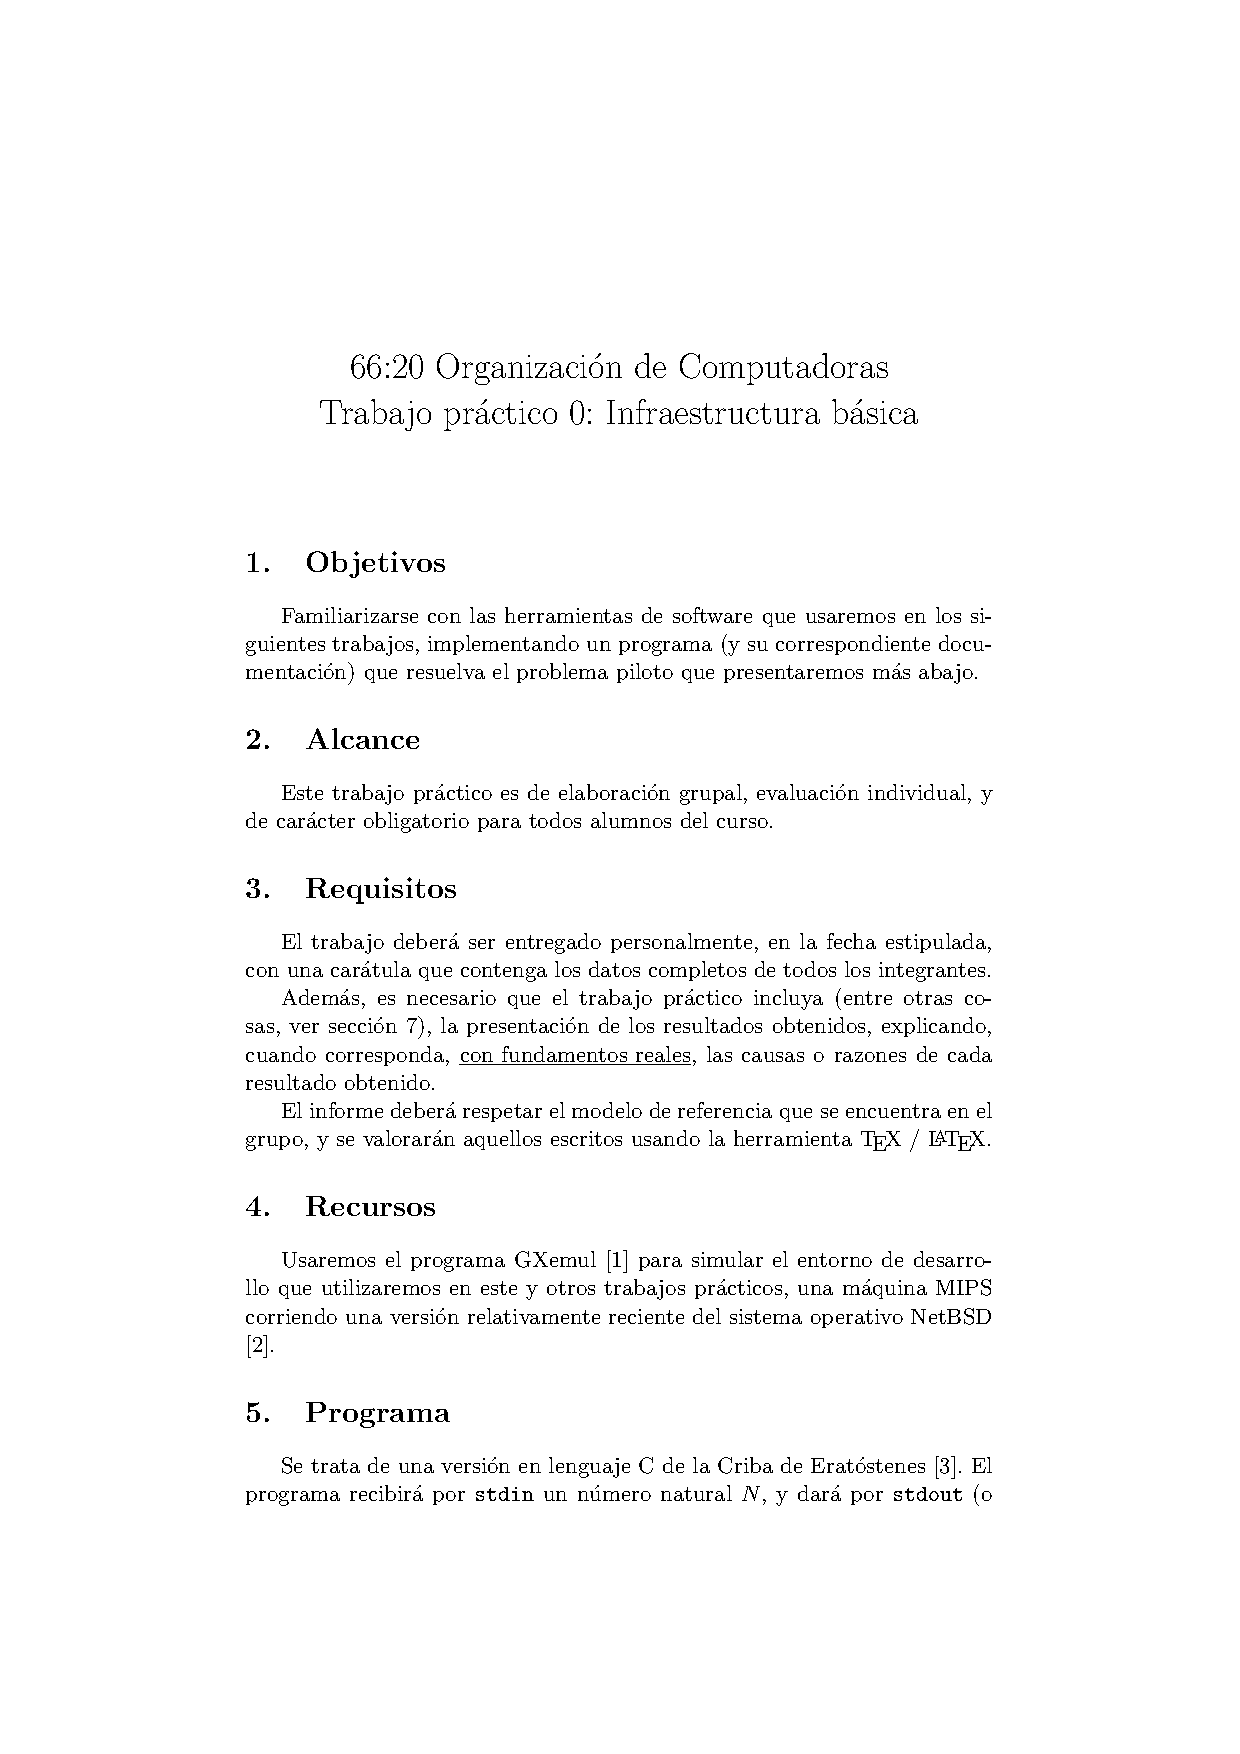
\includepdf[pages=-]{Enunciado.pdf}

\end{document}
